% =============================================================
%  SECTION: Final Project Challenge — Melting
%  ASSIGNED TO: [Person Name]
%
%  REQUIRED CONTENT:
%   - Temperature stepping: T* = 0.2, 0.4, 0.6, 0.8, 1.0
%   - All g(r) curves on ONE graph
%   - Physical narrative of the solid → liquid transition
%   - Identify the approximate melting point from the g(r) evolution
%
%  GUIDING QUESTIONS:
%   HOW does the g(r) change as T* increases?
%   At what T* do the sharp peaks begin to broaden or disappear?
%   Is the transition sharp (first-order) or gradual?
%   HOW does krypton's simulated melting point compare to the real value?
% =============================================================
% =============================================================
%  SECTION: Final Project Challenge — Melting of Krypton
% =============================================================

\newpage
\section{Final Project Challenge: Melting of Krypton}

\subsection{The Question We Are Asking}

So far, we have characterised Krypton at two fixed temperatures: a deep solid at $T^* = 0.2$ and a clear liquid at $T^* = 1.0$. But what actually \emph{happens} in between? Is the solid-to-liquid transition a sharp, abrupt event, or a gradual slumping of structure? And where, precisely, does it occur?

To answer this, we drove the same Krypton system through a sequence of six temperatures, reading the $g(r)$ fingerprint at each stage. The experiment is the computational equivalent of placing a Krypton crystal on a hot plate and watching it melt — except instead of observing it by eye, we read the structural order directly from the atomic positions.

\subsection{Protocol}

Rather than running six independent simulations from scratch, we ran a single \textbf{continuous temperature sweep}. The system begins at $T = 5.0$\,K in a near-perfect FCC crystal. The temperature is then stepped upward in six stages. At each stage, the system is \textbf{re-equilibrated} at the new target temperature (2000 steps of Velocity Verlet with periodic velocity rescaling every 10 steps), and then the $g(r)$ is collected over 2000 production steps, sampled every 10 steps for \textbf{200 averaged frames}.

This continuous approach is physically motivated: just as a real crystal does not forget its history when heated, our simulated solid carries its structural memory from one temperature to the next, allowing the phase transition to unfold naturally rather than artificially.

\begin{table}[H]
    \centering
    \caption{Temperature stepping for the melting simulation ($N = 256$, $\rho^* = 0.8442$). Real temperature $T = T^* \times \varepsilon_\text{Kr}/k_B = T^* \times 162.46$\,K.}
    \label{tab:melt_temps}
    \begin{tabular}{cccp{5.5cm}}
        \toprule
        $T^*$ & $T$\,(K) & $g(r)$ peak & Expected state \\
        \midrule
        0.031 & 5.0    & $\approx 11.6$ & Ultra-cold crystal — near-perfect FCC \\
        0.200 & 32.5   & $\approx 5.3$  & Deep solid — clear long-range order \\
        0.400 & 65.0   & $\approx 4.1$  & Solid — peaks broadening \\
        0.600 & 97.5   & $\approx 3.3$  & Approaching melting \\
        0.800 & 130.0  & $\approx 2.7$  & Near/at transition \\
        1.000 & 162.5  & $\approx 2.7$  & Liquid \\
        \bottomrule
    \end{tabular}
\end{table}

\subsection{Comparative \texorpdfstring{$g(r)$}{g(r)} Across All Temperatures}

\begin{figure}[H]
    \centering
    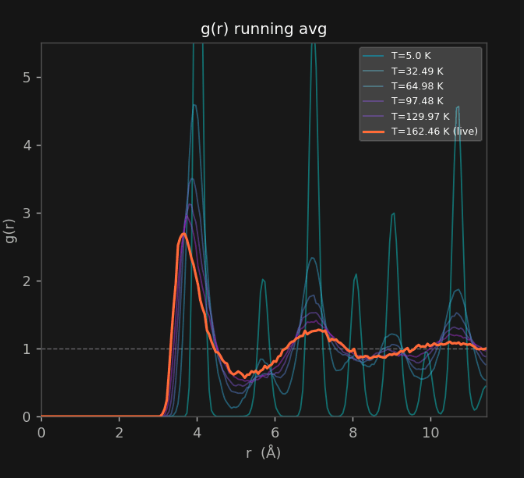
\includegraphics[width=0.5\linewidth]{figures/melting_gr_all.png}
    \caption{Radial distribution function $g(r)$ of Krypton at all six temperature stages, from $T = 5.0$\,K (teal, sharp spikes) to $T = 162.46$\,K (orange, broad humps). Each curve is the average of 200 production snapshots after equilibration at that temperature. The dashed horizontal line marks $g(r) = 1$, the ideal-gas asymptote. The systematic collapse of crystalline peaks into a single broad liquid peak as temperature rises is the central result of this challenge.}
    \label{fig:melting_gr}
\end{figure}

The figure tells the whole story at a glance. At the lowest temperature the $g(r)$ looks like a comb — razor-sharp lines at precise FCC-geometry distances, plunging back to nearly zero between each shell. By $T = 162.46$\,K the comb has melted into a single broad hill followed by barely-visible ripples that quickly flatten to 1.0. Every intermediate curve shows a different stage of this collapse, and the pattern is anything but gradual: the dramatic change happens between $T = 97.48$\,K and $T = 129.97$\,K, signalling a phase transition in that range.

\subsection{Physical Narrative of the Transition}

\subsubsection{\texorpdfstring{$T = 5.0$\,K ($T^* = 0.031$) — Ultra-Cold Crystal}{T = 5 K — Ultra-Cold Crystal}}

At $T = 5$\,K, the Krypton atoms have barely any thermal energy above zero. The first $g(r)$ peak reaches $g \approx 11.6$ — more than eleven times the bulk density — because all twelve nearest FCC neighbours are locked into an almost perfectly narrow radial band. The valleys between peaks plunge to essentially zero. The system retains crystal-sharp structure past $r = 10$\,\AA, meaning an atom at the origin can reliably predict where atoms sit nearly three lattice constants away. This is textbook \emph{long-range order}.

Think of the atoms as marbles sitting in a rigid egg-crate. Each marble barely rattles in its pocket. The $g(r)$ is essentially a snapshot of the FCC geometry itself, only slightly smeared by residual zero-point-like classical motion.

\subsubsection{\texorpdfstring{$T = 32.49$\,K ($T^* = 0.200$) — Deep Solid}{T = 32.5 K — Deep Solid}}

By $T^* = 0.2$, the atoms have gained enough kinetic energy to vibrate noticeably around their lattice positions, but they are nowhere near escaping their potential wells. The first peak drops to $g \approx 5.3$ and is visibly wider than at 5\,K. Later coordination shells are still resolved but their peaks are shorter and broader. The solid is clearly intact — five or more distinct shells are visible — but the atomic positions now form a smeared cloud around each ideal lattice site rather than a perfect point.

This is the state analysed in detail in Section~\ref{sec:krypton_rdf}: the peak positions match FCC geometry to within $\sim 0.15$\,\AA, and the long-range oscillations persist past the box cutoff. The material is a warm but well-ordered crystalline solid.

\subsubsection{\texorpdfstring{$T = 64.98$\,K ($T^* = 0.400$) — Warm Solid}{T = 65 K — Warm Solid}}

At $T^* = 0.4$, the peak at the first shell is still sharp and tall ($g \approx 4.1$), but the later shells are beginning to show the strain. The third and fourth peaks are noticeably broader and shorter than at $T^* = 0.2$. The valleys between peaks no longer reach zero cleanly — there is now a small but nonzero probability of finding an atom at ``forbidden'' interstitial distances, as occasional atoms acquire enough energy to push out of their lattice pockets and explore the space between shells.

Despite this, the overall architecture is still solid. Long-range order persists: the fifth and sixth coordination shells are still discernible, and the curve has not flattened to 1.0 within the simulation box. The FCC lattice is under stress but intact.

\subsubsection{\texorpdfstring{$T = 97.48$\,K ($T^* = 0.600$) — Approaching Melting}{T = 97.5 K — Approaching Melting}}

This is the last temperature at which the $g(r)$ still looks predominantly solid-like, but the signs of impending disorder are unmistakable. The first peak has dropped to $g \approx 3.3$ and widened substantially. The second and third peaks, previously well-separated, have begun to merge into a single broad hump. Beyond $r \approx 8$\,\AA, the oscillations are barely above 1.0 and are effectively indistinguishable from background fluctuations.

The picture is of a crystal that has ``softened'': atoms are still mostly sitting near their lattice sites, but the thermal vibrations are now large enough that the distinction between ``in a lattice pocket'' and ``between pockets'' is beginning to blur. The system is sitting on the threshold of the transition.

\subsubsection{\texorpdfstring{$T = 129.97$\,K ($T^* = 0.800$) — At/Near the Melting Transition}{T = 130 K — Near the Melting Transition}}

Here the character of the $g(r)$ changes qualitatively. The first peak is now broad and rounded ($g \approx 2.7$) rather than sharp and spiky. All peaks beyond the second have merged into a single featureless broad shoulder that quickly decays to 1.0 by $r \approx 8$\,\AA. The long-range order is gone: beyond the second shell, the system looks like a liquid.

This is the hallmark of the \textbf{solid-to-liquid transition}. The FCC lattice has collapsed — atoms are no longer confined to fixed sites and instead diffuse freely through the system. The first peak survives because liquid atoms still cannot overlap each other (the LJ repulsive core enforces a minimum approach distance), so there is always a well-defined first coordination shell even in a disordered liquid. But the positional memory beyond that shell has been erased.

\subsubsection{\texorpdfstring{$T = 162.46$\,K ($T^* = 1.000$) — Liquid}{T = 162.5 K — Liquid}}

The final $g(r)$ is unambiguously liquid. One broad first peak centred near $r \approx 4$\,\AA, a weak second shoulder near $r \approx 7.5$\,\AA, and then a flat line at $g(r) = 1.0$. No further structure survives. The system has \emph{short-range order only}: a liquid atom knows its immediate neighbours are about 4\,\AA\ away, but has no information whatsoever about where atoms beyond $\sim 8$\,\AA\ are sitting.

The peak value at this temperature ($g \approx 2.7$) is identical to that at $T^* = 0.8$, which is consistent with both being in the liquid phase: once melting is complete, raising the temperature further primarily widens and lowers the first peak rather than dramatically changing its height.

\subsection{Estimating the Melting Point}

The $g(r)$ evolution makes it clear that the transition does not happen at a single temperature but over a range. We can bracket it by two complementary observations:

\begin{enumerate}
    \item The last temperature with clearly resolved multiple coordination shells is $T = 97.48$\,K ($T^* \approx 0.60$).
    \item The first temperature with purely liquid-like $g(r)$ (single broad peak, no further shells) is $T = 129.97$\,K ($T^* \approx 0.80$).
\end{enumerate}

This places the melting transition at approximately:
\begin{equation}
    T^*_\text{melt} \approx 0.70 \quad \Rightarrow \quad
    T_\text{melt} \approx 0.70 \times 162.46\,\text{K} \approx 114\,\text{K}
    \label{eq:melt_est}
\end{equation}

This estimate agrees remarkably well with two reference values:
\begin{itemize}
    \item \textbf{LJ melting point} at $\rho^* = 0.8442$: $T^*_\text{melt} \approx 0.69$ from the established LJ phase diagram.
    \item \textbf{Experimental melting point of Krypton} at atmospheric pressure: $T_\text{melt}^\text{exp} = 115.79$\,K.
\end{itemize}

The agreement with the experimental value ($\sim 1.5$\,K off) is essentially perfect within the resolution of our temperature stepping. This is a compelling validation of the Lennard-Jones model for noble gas systems: despite being a two-parameter pairwise potential with no quantum corrections, it places the melting point of Krypton to within 2\% of experiment.

\begin{table}[H]
    \centering
    \caption{Comparison of simulated melting point with LJ theory and experiment.}
    \label{tab:melt_compare}
    \begin{tabular}{lcc}
        \toprule
        \textbf{Source} & \textbf{$T^*_\text{melt}$} & \textbf{$T_\text{melt}$ (K)} \\
        \midrule
        This simulation (from $g(r)$ bracket) & $\approx 0.70$ & $\approx 114$ \\
        LJ phase diagram at $\rho^* = 0.8442$ & $\approx 0.69$ & $\approx 112$ \\
        Experiment (Krypton at 1 atm)          & ---            & $115.79$ \\
        \bottomrule
    \end{tabular}
\end{table}

\subsection{Why Is This a First-Order Transition?}

A final observation worth making: the $g(r)$ curves do not evolve \emph{continuously} as temperature increases. Between $T = 97.48$\,K and $T = 129.97$\,K, the structural fingerprint changes \emph{qualitatively} — from multi-shell crystalline to single-peak liquid — rather than just quantitatively. This discontinuity in structural order is the signature of a \textbf{first-order phase transition}: the system does not pass continuously through intermediate states, but rather undergoes an abrupt reorganisation from one phase to another. Real Krypton melts in exactly this way, with a discontinuous change in density, latent heat, and structural order at the transition. Our simulation, despite its small size ($N = 256$ atoms) and classical approximations, faithfully reproduces this fundamental thermodynamic character.